\documentclass{article}
\usepackage[utf8]{inputenc} % For proper handling of UTF-8 characters
\usepackage{amsmath}        % For advanced mathematical typesetting
\usepackage{amssymb}        % For additional mathematical symbols
\usepackage{amsthm}         % For theorem-like environments (though not used for solutions here)
\usepackage{graphicx}       % For including images (implicitly used by pgfplots, good to have)
\usepackage{pgfplots}       % For creating plots and graphs
\pgfplotsset{compat=1.18}    % Ensure compatibility with a recent PGFPlots version
\usepackage{hyperref}       % For creating hyperlinks in the document
\usepackage{enumitem}       % For customizing list environments
\usepackage{xcolor}         % For colored text (not strictly used, but harmless)

% Custom commands for lesson structure
\newcommand{\lessonsection}[1]{\section*{#1}}
\newcommand{\lessonsubsection}[1]{\subsection*{#1}}
\newcommand{\example}[1]{\lessonsubsection{Worked Example: #1}}
\newcommand{\exercise}[1]{\lessonsubsection{Exercises: #1}}

\begin{document}

\title{The Evolution of Artificial Intelligence: A Journey Through Time}
\author{Academic LaTeX Expert}
\date{\today}

\maketitle

\begin{abstract}
This lesson provides a comprehensive overview of the historical evolution of Artificial Intelligence (AI), tracing its origins from early philosophical concepts and foundational theories to the modern era of deep learning and large language models. We explore key milestones, pivotal breakthroughs, periods of stagnation (AI Winters), and the underlying technological and conceptual shifts that have shaped the field. The lesson includes a conceptual explanation, a worked example illustrating an early AI paradigm, and a set of three-level exercises to reinforce understanding.
\end{abstract}

\lessonsection{Introduction}
Artificial Intelligence (AI) is a rapidly evolving field dedicated to creating machines that can perform tasks typically requiring human intelligence. From its theoretical inception to its current pervasive influence, AI's journey has been marked by cycles of immense optimism, significant breakthroughs, and periods of disillusionment. Understanding this evolution is crucial for appreciating the current state of AI and anticipating its future trajectory. This lesson will guide you through the key phases of AI development, highlighting the foundational ideas, technological advancements, and paradigm shifts that have defined its history.

\lessonsection{Concept Explanation: A Timeline of AI Evolution}

\lessonsubsection{1. Early Foundations and Theoretical Beginnings (1940s-1950s)}
The seeds of AI were sown in the mid-20th century, driven by advancements in logic, computation, and cognitive science.
\begin{itemize}
    \item \textbf{1943:} Warren McCulloch and Walter Pitts publish "A Logical Calculus of Ideas Immanent in Nervous Activity," proposing the first mathematical model of an artificial neuron.
    \item \textbf{1950:} Alan Turing publishes "Computing Machinery and Intelligence," introducing the \textbf{Turing Test} as a criterion for machine intelligence and laying philosophical groundwork.
    \item \textbf{1956:} The \textbf{Dartmouth Workshop}, organized by John McCarthy, Marvin Minsky, Nathaniel Rochester, and Claude Shannon, formally coins the term "Artificial Intelligence" and marks the birth of AI as a distinct academic discipline. Early work focused on symbolic reasoning and problem-solving.
    \item \textbf{1956:} Allen Newell and Herbert A. Simon develop the \textbf{Logic Theorist}, considered the first AI program, capable of proving mathematical theorems.
\end{itemize}

\lessonsubsection{2. The Golden Age of AI and Early Enthusiasm (1950s-1960s)}
This period saw significant optimism and initial successes in symbolic AI.
\begin{itemize}
    \item \textbf{1959:} Arthur Samuel develops a checkers-playing program that learns from its own experience, demonstrating early machine learning concepts.
    \item \textbf{1961:} James Slagle's SAINT program solves calculus problems.
    \item \textbf{1965:} Joseph Weizenbaum creates \textbf{ELIZA}, an early natural language processing program that simulated a Rogerian psychotherapist, demonstrating the power of simple pattern matching.
    \item \textbf{1969:} Marvin Minsky and Seymour Papert publish "Perceptrons," highlighting limitations of single-layer neural networks, which contributed to a decline in neural network research for a period.
\end{itemize}

\lessonsubsection{3. The First AI Winter (1970s)}
Over-optimism and the inability of early AI systems to scale beyond "toy problems" led to disillusionment and significant funding cuts.
\begin{itemize}
    \item Limitations of symbolic AI in handling real-world complexity and ambiguity became apparent.
    \item The "frame problem" and "common sense knowledge" proved difficult to formalize.
    \item Lighthill Report (1973) in the UK was highly critical, leading to reduced government funding.
\end{itemize}

\lessonsubsection{4. Expert Systems and the AI Revival (1980s)}
A new paradigm emerged, focusing on knowledge-based systems that encoded human expertise in specific domains.
\begin{itemize}
    \item \textbf{Expert Systems} like DENDRAL (for chemical structure analysis), MYCIN (for diagnosing infectious diseases), and R1/XCON (for configuring VAX computer systems) achieved commercial success.
    \item These systems used rule-based reasoning (e.g., IF-THEN rules) and inference engines.
    \item Japan's Fifth Generation Computer Systems project (FGCS) fueled significant investment and research.
\end{itemize}

\lessonsubsection{5. The Second AI Winter (Late 1980s-Early 1990s)}
The high cost of developing and maintaining expert systems, their brittleness (inability to handle situations outside their knowledge base), and the collapse of the Lisp machine market led to another period of reduced interest and funding.

\lessonsubsection{6. Machine Learning and Data-Driven AI (1990s-2000s)}
A shift from symbolic, rule-based AI to statistical and data-driven approaches marked this era.
\begin{itemize}
    \item Focus on algorithms that could learn from data, rather than being explicitly programmed with rules.
    \item Rise of algorithms like \textbf{Support Vector Machines (SVMs)}, Decision Trees, and Bayesian Networks.
    \item Increased availability of data and computational power made these approaches viable.
    \item \textbf{1997:} IBM's Deep Blue defeats world chess champion Garry Kasparov, a landmark achievement in search algorithms and specialized hardware.
\end{itemize}

\lessonsubsection{7. The Deep Learning Revolution (2010s-Present)}
This period is characterized by the resurgence of neural networks, particularly deep neural networks, fueled by massive datasets, powerful GPUs, and algorithmic innovations.
\begin{itemize}
    \item \textbf{2012:} AlexNet wins the ImageNet Large Scale Visual Recognition Challenge (ILSVRC), significantly outperforming previous methods and sparking widespread interest in deep learning.
    \item Breakthroughs in areas like computer vision (CNNs), natural language processing (RNNs, Transformers), and speech recognition.
    \item \textbf{2016:} AlphaGo, a program developed by DeepMind, defeats world champion Go player Lee Sedol, a game considered far more complex than chess for AI.
    \item Development of \textbf{Large Language Models (LLMs)} like GPT-3, BERT, and their successors, demonstrating unprecedented capabilities in natural language understanding and generation.
    \item AI becomes integrated into countless applications, from recommendation systems to autonomous vehicles.
\end{itemize}

\lessonsubsection{8. Future Directions}
The field continues to evolve rapidly, with ongoing research into:
\begin{itemize}
    \item \textbf{Artificial General Intelligence (AGI):} Creating AI that can perform any intellectual task a human can.
    \item \textbf{Explainable AI (XAI):} Making AI decisions transparent and understandable.
    \item \textbf{Ethical AI:} Addressing bias, fairness, privacy, and societal impact.
    \item \textbf{Reinforcement Learning:} Further advancements in agents learning through interaction with environments.
\end{itemize}

\begin{figure}[htbp]htbp] % Placement specifier [htbp] applied exactly as requested
    \centering
    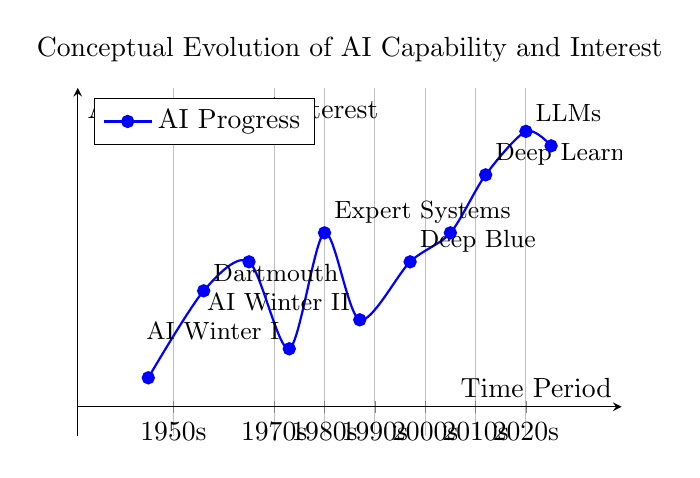
\begin{tikzpicture}
        \begin{axis}[
            axis lines=middle,
            enlargelimits,
            width=0.7\textwidth, % Scaling set to 0.7\textwidth as requested
            height=6cm,
            xlabel={Time Period},
            ylabel={AI Capability / Interest},
            xmin=1940, xmax=2030,
            ymin=0, ymax=10,
            xtick={1950, 1970, 1980, 1990, 2000, 2010, 2020},
            xticklabels={1950s, 1970s, 1980s, 1990s, 2000s, 2010s, 2020s},
            ytick=\empty, % No y-axis ticks, just conceptual curve
            grid=major,
            title={Conceptual Evolution of AI Capability and Interest},
            legend pos=north west
        ]
            \addplot[smooth, thick, blue, mark=*, mark options={fill=blue}] coordinates {
                (1945, 1) % Pre-AI
                (1956, 4) % Dartmouth, early enthusiasm
                (1965, 5) % ELIZA, early successes
                (1973, 2) % AI Winter I (Lighthill Report)
                (1980, 6) % Expert Systems boom
                (1987, 3) % AI Winter II (Expert Systems limitations)
                (1997, 5) % Deep Blue, ML rise
                (2005, 6) % Data-driven ML
                (2012, 8) % Deep Learning revolution (AlexNet)
                (2020, 9.5) % LLMs, current peak
                (2025, 9) % Potential future plateau/challenges
            };
            \addlegendentry{AI Progress}

            % Annotations for key events/periods
            \node[anchor=south west, font=\small] at (axis cs:1956,4) {Dartmouth};
            \node[anchor=south east, font=\small] at (axis cs:1973,2) {AI Winter I};
            \node[anchor=south west, font=\small] at (axis cs:1980,6) {Expert Systems};
            \node[anchor=south east, font=\small] at (axis cs:1987,3) {AI Winter II};
            \node[anchor=south west, font=\small] at (axis cs:1997,5) {Deep Blue};
            \node[anchor=south west, font=\small] at (axis cs:2012,8) {Deep Learning};
            \node[anchor=south west, font=\small] at (axis cs:2020,9.5) {LLMs};

        \end{axis}
    \end{tikzpicture}
    \caption{A conceptual representation of AI capability and public interest over time, illustrating periods of rapid advancement and "AI Winters."}
    \label{fig:ai_evolution_graph}
\end{figure}

\example{A Simplified Expert System for Medical Diagnosis}
Let's consider a very basic expert system designed to assist in diagnosing a simple medical condition based on symptoms. This example illustrates the rule-based approach prevalent during the 1980s.

\textbf{Scenario:} A patient presents with symptoms, and the system needs to suggest a possible diagnosis.

\textbf{Knowledge Base (Rules):}
\begin{enumerate}
    \item \texttt{IF (Symptom = "fever") AND (Symptom = "cough") THEN (Condition = "common cold")}
    \item \texttt{IF (Symptom = "fever") AND (Symptom = "rash") THEN (Condition = "measles")}
    \item \texttt{IF (Symptom = "cough") AND (Symptom = "shortness of breath") THEN (Condition = "bronchitis")}
    \item \texttt{IF (Condition = "common cold") THEN (Treatment = "rest and fluids")}
    \item \texttt{IF (Condition = "measles") THEN (Treatment = "vaccination history check")}
\end{enumerate}

\textbf{Inference Engine (Reasoning Process):}
Suppose a patient reports: \texttt{Symptom = "fever"} and \texttt{Symptom = "cough"}.

\begin{enumerate}
    \item The inference engine scans the knowledge base for rules whose conditions match the observed symptoms.
    \item Rule 1: \texttt{IF (Symptom = "fever") AND (Symptom = "cough")} matches.
    \item \textbf{Conclusion 1:} The system infers \texttt{(Condition = "common cold")}.
    \item Now, with \texttt{(Condition = "common cold")} established, the inference engine looks for rules that use this as a premise.
    \item Rule 4: \texttt{IF (Condition = "common cold")} matches.
    \item \textbf{Conclusion 2:} The system infers \texttt{(Treatment = "rest and fluids")}.
\end{enumerate}

\textbf{Output:} Based on the symptoms, the system suggests "common cold" as a possible condition and "rest and fluids" as a recommended treatment.

\textbf{Significance:}
This example demonstrates how expert systems could mimic human decision-making in narrow domains by explicitly encoding knowledge and rules. While powerful for their time, their limitations included difficulty in acquiring and maintaining large knowledge bases, lack of common sense, and inability to learn from new data without manual rule updates. This brittleness ultimately contributed to the second AI Winter.

\exercise{Test Your Knowledge}

\begin{enumerate}[label=\textbf{Q\arabic*.}, ref=Q\arabic*]
    \item \textbf{Level 1: Recall}
    What was the primary purpose of the Dartmouth Workshop in 1956, and what significant term was coined there?

    \textbf{Solution:}
    The primary purpose of the Dartmouth Workshop in 1956 was to bring together researchers interested in "thinking machines" and to formally establish the field. It is widely recognized as the birth of Artificial Intelligence as an academic discipline. The significant term coined at this workshop was "Artificial Intelligence" itself.

    \item \textbf{Level 2: Application/Analysis}
    Explain the concept of an "AI Winter." Describe two distinct factors that contributed to the first AI Winter in the 1970s.

    \textbf{Hint:} Consider the limitations of the AI paradigms prevalent at the time (e.g., symbolic AI's struggle with real-world complexity) and external influences on research funding (e.g., critical reports).

    \item \textbf{Level 3: Critical Thinking/Synthesis}
    The Deep Learning revolution of the 2010s was fueled by three major converging factors. Identify these factors and explain how their synergy enabled the unprecedented success of deep learning compared to earlier neural network research. Discuss one potential challenge or ethical consideration that arises from the widespread adoption of deep learning models today.
\end{enumerate}

\end{document}